\documentclass[12pt]{article}

\usepackage{graphicx,url}
%\usepackage[latin1]{inputenc}  
\usepackage[utf8]{inputenc}  
\usepackage[brazil]{babel}
\usepackage{float}
% UTF-8 encoding is recommended by ShareLaTex
     
\sloppy

\title{Micro-arquitetura ZEN e sua implementação no Ryzen 7}

\author{Roberto Gonçalves Santos Júnior \and João Francisco de Oliveira Batista 
\and Leonardo Carvalho de Oliveira \and Guilherme Bertoluchi \and Gustavo Nunes \and Marcos Oliveira}


\address{
\centering
Departamento de Ciência da Computação \\ Universidade Federal de Lavras
  (UFLA)\\ Caixa Postal 15.064 -- 91.501-970 \\ Lavras, MG -- Brazil \\
\nextinstitute
  Departamento de Ciência da Computação\\
  Universidade Federal de Lavras \\ Lavras, MG -- Brazil \\
  \email{
  \{roberto.goncalves\}@computacao.ufla.br, {jonesjoao}@computacao.ufla.br, \\{leo}@computacao.ufla.br}
}

\thispagestyle{empty}
\newpage


\begin{document} 

\maketitle
\thispagestyle{empty}
\newpage

\tableofcontents
\thispagestyle{empty}
\newpage

\begin{abstract}
  This paper describes a technical analysis about the ZEN microarchitecture provided by AMD. This analysis consists on the each block of ZEN architecture and their detailed description about how it works. Futhermore, discuss what has been implemented on Ryzen 7.
\end{abstract}

\begin{resumo}
  Esse artigo descreve a analise técnica sobre a microarquitetura ZEN desenvolvida pela AMD. Essa analise consiste na separação de cada bloco da arquitetura ZEN e sua descrição detalhada de como ela funciona. Além disso, discutir o que foi implementado no Ryzen 7. 
\end{resumo}

\thispagestyle{empty}
\newpage

\section{Hierarquia de Memória}
A mais importante novidade relacionada a memória na microarquitetura Zen é a introdução de um novo sistema de cache de baixa latência com grande largura de banda, ou seja, uma cache com uma ICP muito melhor, pois mais instruções serão executadas em menor tempo. Este elemento é essencial para a performance de um processador com múltiplos núcleos que pretende usar o multithread de forma eficiente.
Agora cada núcleo Zen inclui uma nova cache de micro operações.
Ela terá suporte tanto à DDR3 quanto DDR4.Como a zen é baseada em um unidade quad core, cada núcleo dela terá um cache L3 compartilhada de 8MB em um total de quatro cores, uma dedicada cache L2 de 512KB . Como já dito, ela foi projetada para um alta performance e uma baixa potência.Tal cache L3 é 16-way associative, e exclusiva da cache L2.

\begin{figure}[h!]
\centering
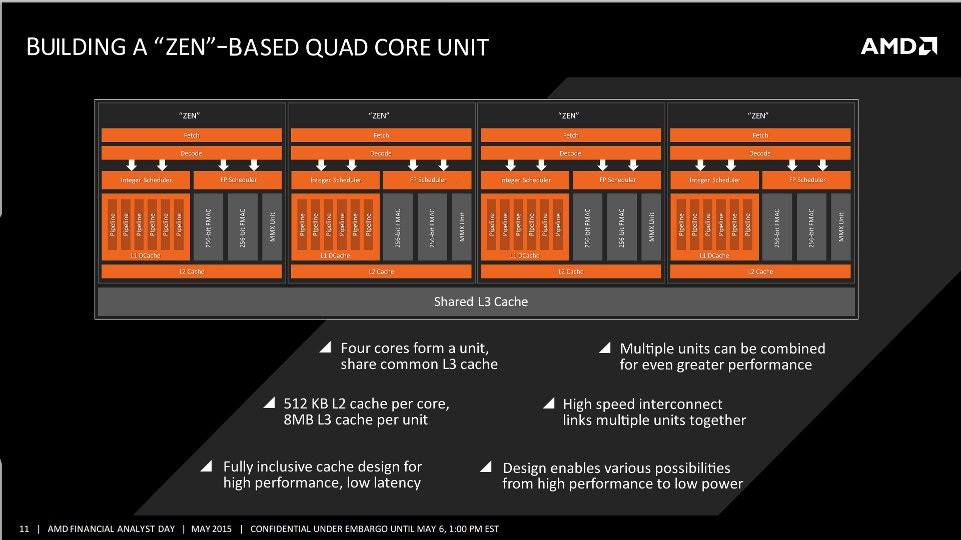
\includegraphics[width=120mm,scale=0.8]{amd.jpg}
\caption{Construção do Zen baseado no quad core unit , fonte: AMD}
\label{fig:amd}
\end{figure}

buffers muito mais amplos internos
Como é uma unidade quad core, os cores não compartilham nada além desse cache L3, sendo assim independentes. Dizem que tal característica resulta em melhores núcleos em relação à performance e eficiência.

Na ideia da Zen também foi incluído um sistema de cache muito melhor, como Write back na cache L1, diferenciando dos Bulldozer que usavam Write Through. Uma cache L2 e uma cache L3 e uma FPU mais rápida, sendo uma cache L2 e FPU privadas, e com uma quantidade de buffers internos maior. As larguras de banda das memórias cache também aumentaram.

\begin{figure}[h!]
\centering
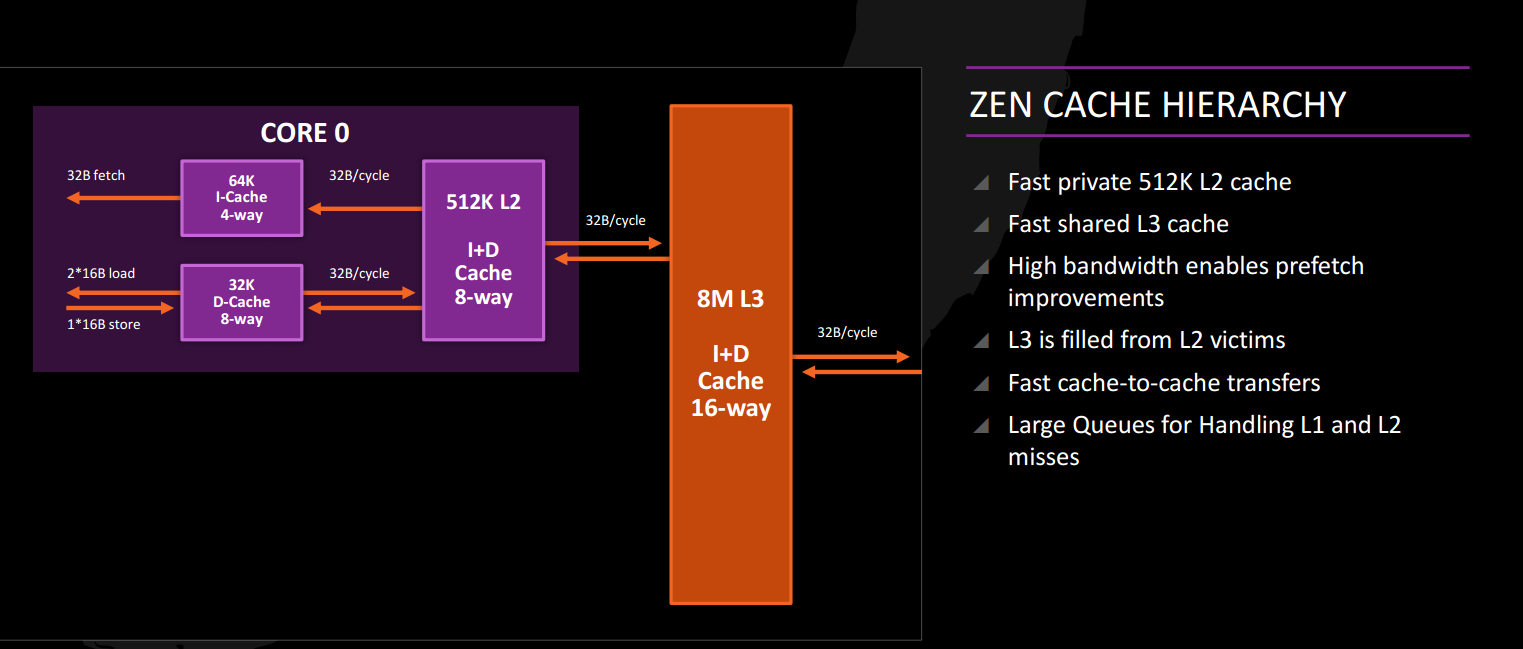
\includegraphics[width=120mm,scale=0.8]{ZenCache.png}
\caption{Hierarquia de cache no Zen, fonte: AMD}
\label{fig:amd}
\end{figure}
Isso fez com os processadores AMD Zen,trabalhem de forma paralela e mais efetiva em relação a seus produtos antigos, e visando um futuro de seus concorrentes, portanto a amd conseguiu fazer com que sua nova arquitetura resultasse em melhores núcleos tanto em termos de performance quanto de eficiência.

\newpage

\section{Cache de micro-operações}

O processador Ryzen 7 é o primeiro processador da AMD a utilizar da tecnologia da cache de micro operações, o que resultava na sua perda de mercado constante contra a Intel assim a AMD teve que correr atrás do prejuízo.

\begin{figure}[H]
\centering
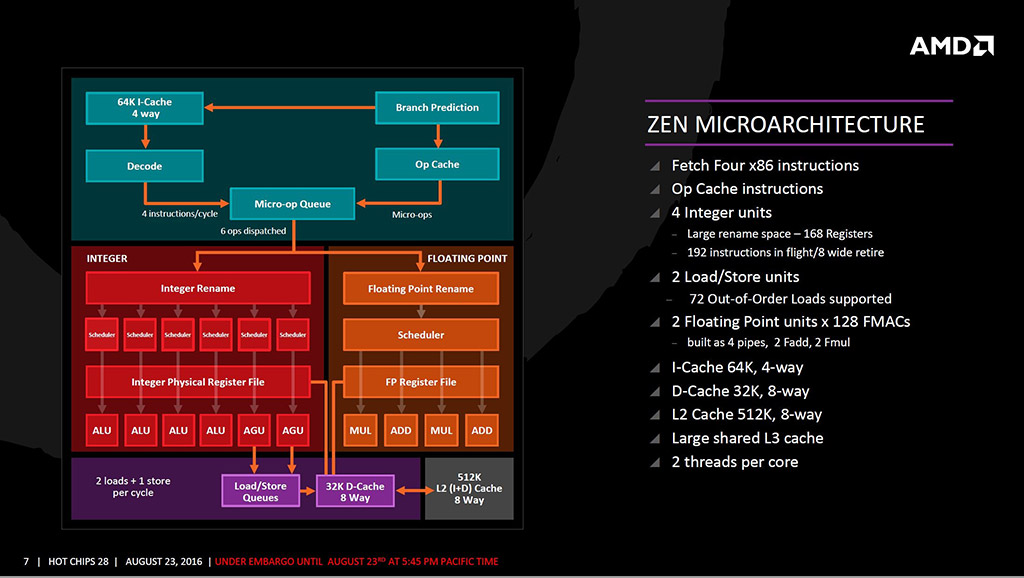
\includegraphics[width=120mm,scale=0.8]{micro-op_cache.jpg}
\caption{Micro-Arquitetura ZEN, fonte: AMD}
\label{fig:AMD CORE}
\end{figure}

O núcleo Zen é uma microarquitetura dramaticamente melhor do que a geração anterior, a Bulldozer. O projeto do Bulldozer da AMD não tinha nenhuma cache de operação, isso fazia com que ele obtivesse detalhes de outras caches para implementar micro-operações usadas com frequência.

Agora cada núcleo Zen inclui uma nova cache de micro operações e uma cache de dados L1 que utiliza o write-back, diferentemente da sua geração anterior que utilizava uma cache de write-through, que foi uma fonte de muito tempo ocioso em algumas partes de códigos, que tem maior desempenho e menor consumo. Ele tem multithreading bidirecional e buffers muito mais amplos internos, com FP privado e unidades SIMD, bem como um cache L2 privado.

Além disso, a AMD disse que o decodificador do Zen, neste momento, pode decodificar quatro instruções por ciclo para encher a fila de operações. Essa fila, com a ajuda do cache de micro operações, pode fornecer até 6 operações/ciclo para os agendadores, porém em média são fornecidas 4 operações uma vez que uma instrução mapeia uma micro operação. Elas ainda são relativamente pequenas, a versão da Intel pode suportar 1536 micro operações com associatividade 8-way. Já a cache de micro-operações para o Zen pode suportar micro-operações de 2K cp, até 8 operações por linha de cache.

A cache de micro-operação pode ser assim determinada como uma cache que armazena micro-operações de instruções recebidas da cache de instrução. Quando uma instrução precisa ser decodificada a cache de micro operações é verificada, quanto ao formato que não foi decodificado, que é reutilizado em armazenamento na cache. Caso não esteja disponível, a instrução será decodificada e armazenada em cache.

A latência que resulta das penalidades de faltas são bastante significativas e uma das opções para aumentar o desempenho por trás dessas penalidades foi acrescentar a cache de micro-operações. A cache de micro operações permite que as instruções que foram recentemente usadas sejam chamadas na fila de micro operações em vez de serem decodificadas novamente, diminuindo assim os acessos através do núcleo e outros níveis de cache, pois com um acerto(hit) nessa nova cache de micro-operações é reduzido o comprimento do pipeline em dois estágios e ainda é cancelado o pedido da cache de instrução L1. A cache de micro operações possui, ainda as micro-tags que são testadas quando uma instrução de ponteiro tem seu endereço físico determinada, entrando assim em uma fila de solicitações da cache convencional. Então, as micro-tags indicam se um determinado endereço está presente ou não, e se estiver, qual modo de cache é prevista para conter as micro-operações desejadas.

\begin{figure}[H]
\centering
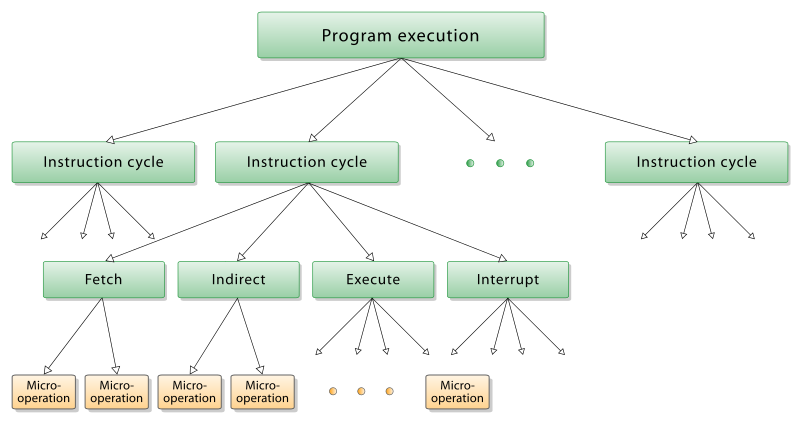
\includegraphics[width=115mm,scale=0.8]{Micro-operations.png}
\caption{Ilustração da decomposição em várias micro-operações}
\label{fig:AMD CORE}
\end{figure}

É importante ressaltar ainda que, quem controla a execução das micro operações é a unidade de controle da CPU, que decide sobre a sua execução ao executar várias otimizações, como por exemplo, reordenamento, fusão e cache.

\newpage

\section{A arquitetura ZEN no Ryzen 7}

A arquitetura ZEN é muito diferente das antigas arquiteturas da AMD, e segundo a AMD, com ela, eles conseguiram alcançar "40\% IPC(Instructions per clock) speedup em relação a arquitetura do  Excavator" o que nessa seção, será discutido no Ryzen 7 1700.\\

\begin{figure}[H]
\centering
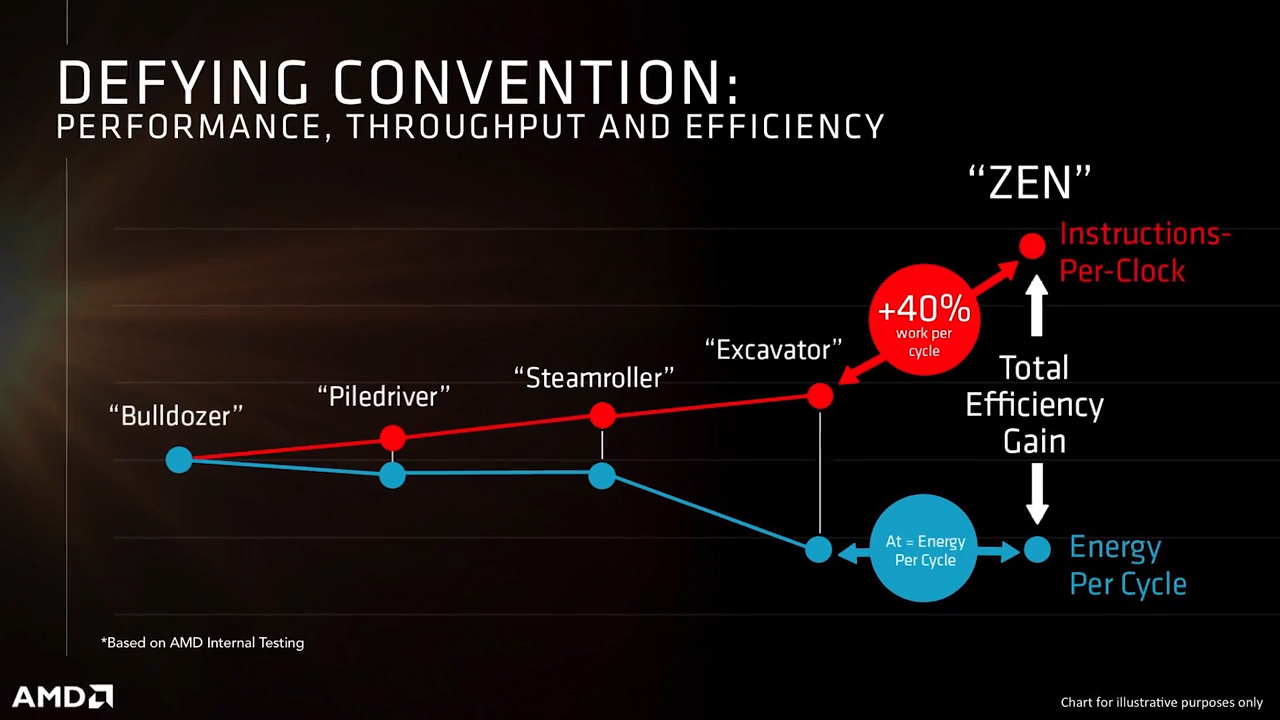
\includegraphics[width=120mm,scale=0.8]{AMD-energy-per-cycle.jpg}
\caption{Comparação ZEN, fonte: AMD}
\label{fig:AMD CORE}
\end{figure}

É importante salientar que segundo o gráfico, houve 40\% ganho de IPC e o mesmo número de energia por ciclo do Excavator, esse é um dos motivos da grande surpresa na arquitetura ZEN.


\begin{figure}[H]
\centering
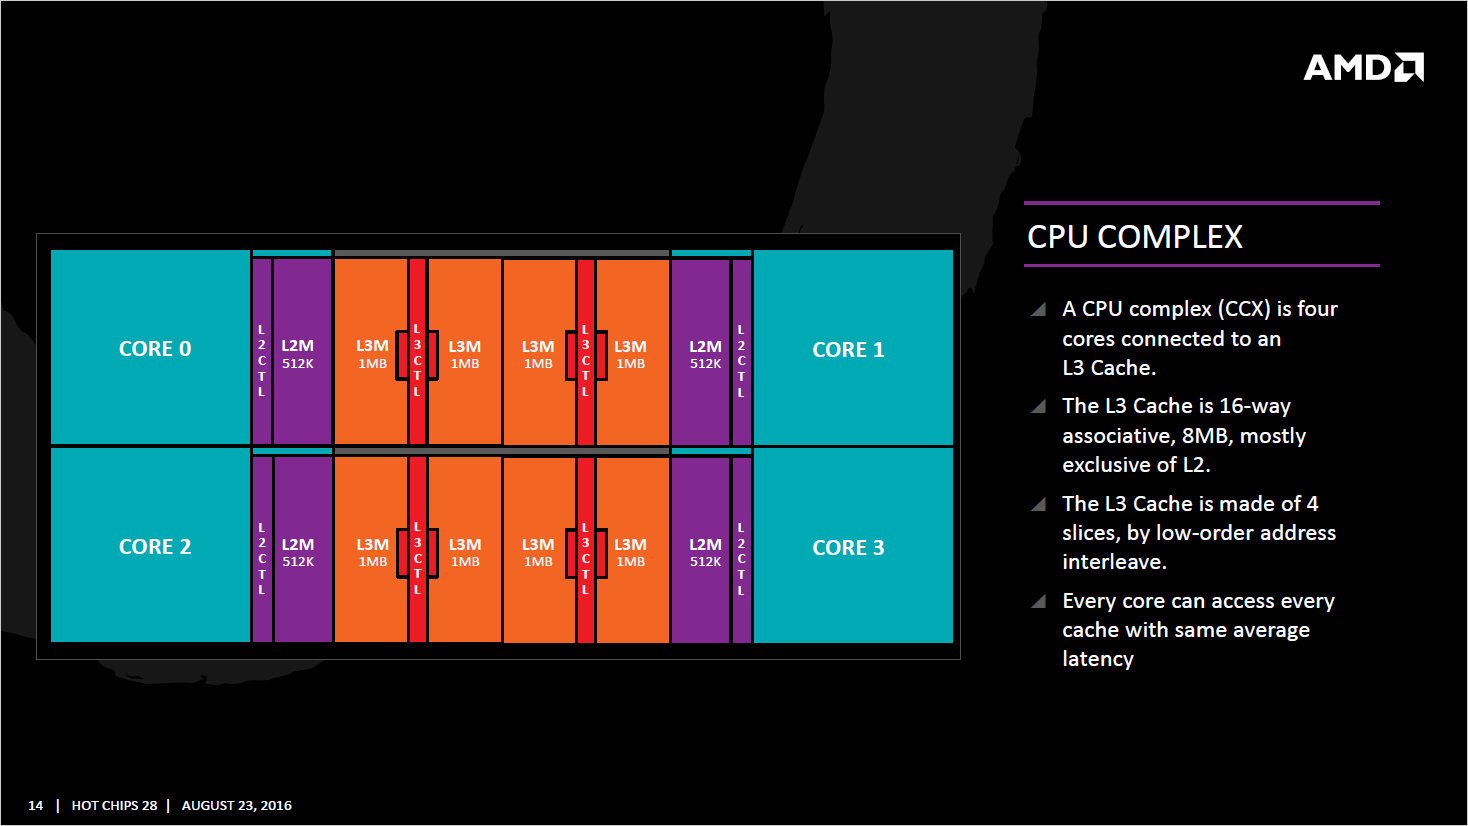
\includegraphics[width=120mm,scale=0.8]{AMD-Zen_CPU-Complex.png}
\caption{CPU Complex, fonte: AMD}
\label{fig:AMD CORE}
\end{figure}

A CPU Complex conhecida como CCX é o conjunto de núcleos da CPU. É importante ressaltar que cada CCX está conectada a uma cache L3. Sendo que, a associatividade da Cache L3 é 16-way, diminuindo o miss rate, e que ela é feita de 4 pedaços, por low-order. E por fim, cada núcleo pode acessar cada cache como a mesma latência média.

Essa mudança foi crucial para o desempenho do Zen sobre o Excavator, na relação em que aumentou-se o número de pipelines de 4 para 6 na cache L1 e houve uma duplicação da quantidade de bits para a FMAC(fused multiply–add capability). Além disso, permaneceu a MMX Unit(Matrix Math Extensions), ou seja, uma unidade auxiliar para efetuar calculos envolvendo matrizes. 

O aumento da duplicação da quantidade de bits para a FMAC, possibilita o aumento da quantidade de instruções que podem ser executadas em cada FMAC. Outra modificação importante é uma instruction decoder para Inteiro e FP, que no Excavator era divida. A unidade de decodificação é responsável, basicamente, por determinar qual instrução será executada depois que passou pelo instruction memory.


\begin{figure}[H]
\centering
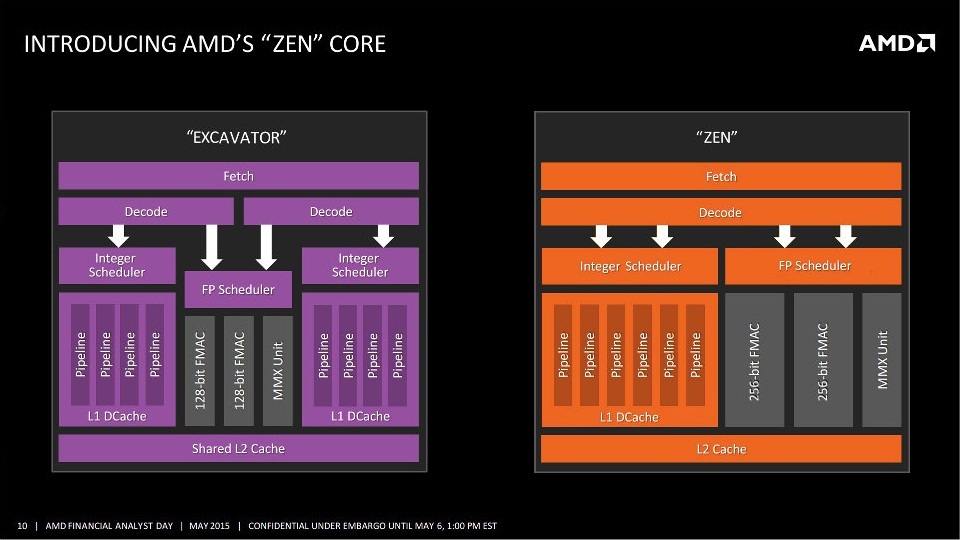
\includegraphics[width=115mm,scale=0.8]{zenex.jpg}
\caption{CPU Complex, fonte: AMD}
\label{fig:AMD CORE}
\end{figure}

A partir dessas informações, com o aumento da capacidade das FMACs, investimento na Cache L3 de cada CCX e o aumento do número de pipelines da cache L1, pode ocorrer que para alguns softwares o IPC do ZEN supere o IPC do Excavator.

A etapa instruction fetch do Pipeline é a primeira etapa do processo, e a arquitetura ZEN tem algumas diferenças das arquiteturas anteriores:

\begin{figure}[H]
\centering
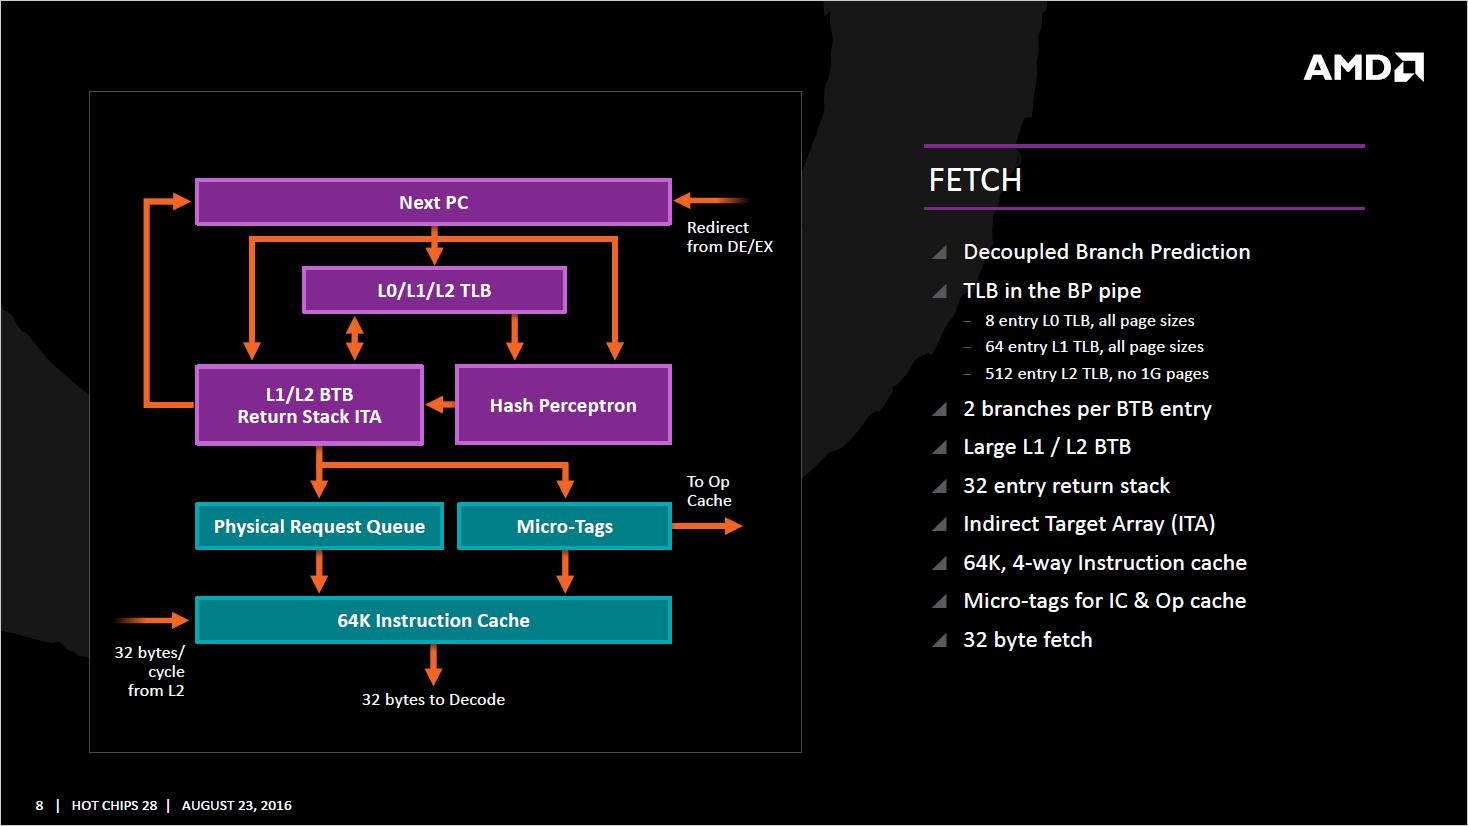
\includegraphics[width=115mm,scale=0.8]{AMD-Zen_Fetch.png}
\caption{CPU Complex, fonte: AMD}
\label{fig:AMD CORE}
\end{figure}

Uma importante inovação da AMD nesse diagrama é o Branch Predictor desacoplado, isso significa que o fetching tem mais liberdade para percorrer outros componentes da CPU, usando alguns algoritmos internos pra CPU. De certa forma, isso irá reduzir a latência da CPU e vai reduzir as bolhas do pipeline, mas caso falhe, terá uma penalidade de poder.

A TLB(Translation Lookaside Buffer) no Branch Predictor é responsável para reduzir a latência armazenando valores de traduções(virtual page - physical page) mais recentes, que está operando em 3 levels:

\begin{itemize}
	\item L0 com 8 entradas de páginas de qualquer tamanho; ?? Perguntar Luiz
	\item L1 com 64 entradas de páginas de qualquer tamanho; ?? Perguntar Luiz
	\item l2 com 512 entradas e suporte pra páginas de 4K até 256K;
\end{itemize}

\begin{figure}[H]
\centering
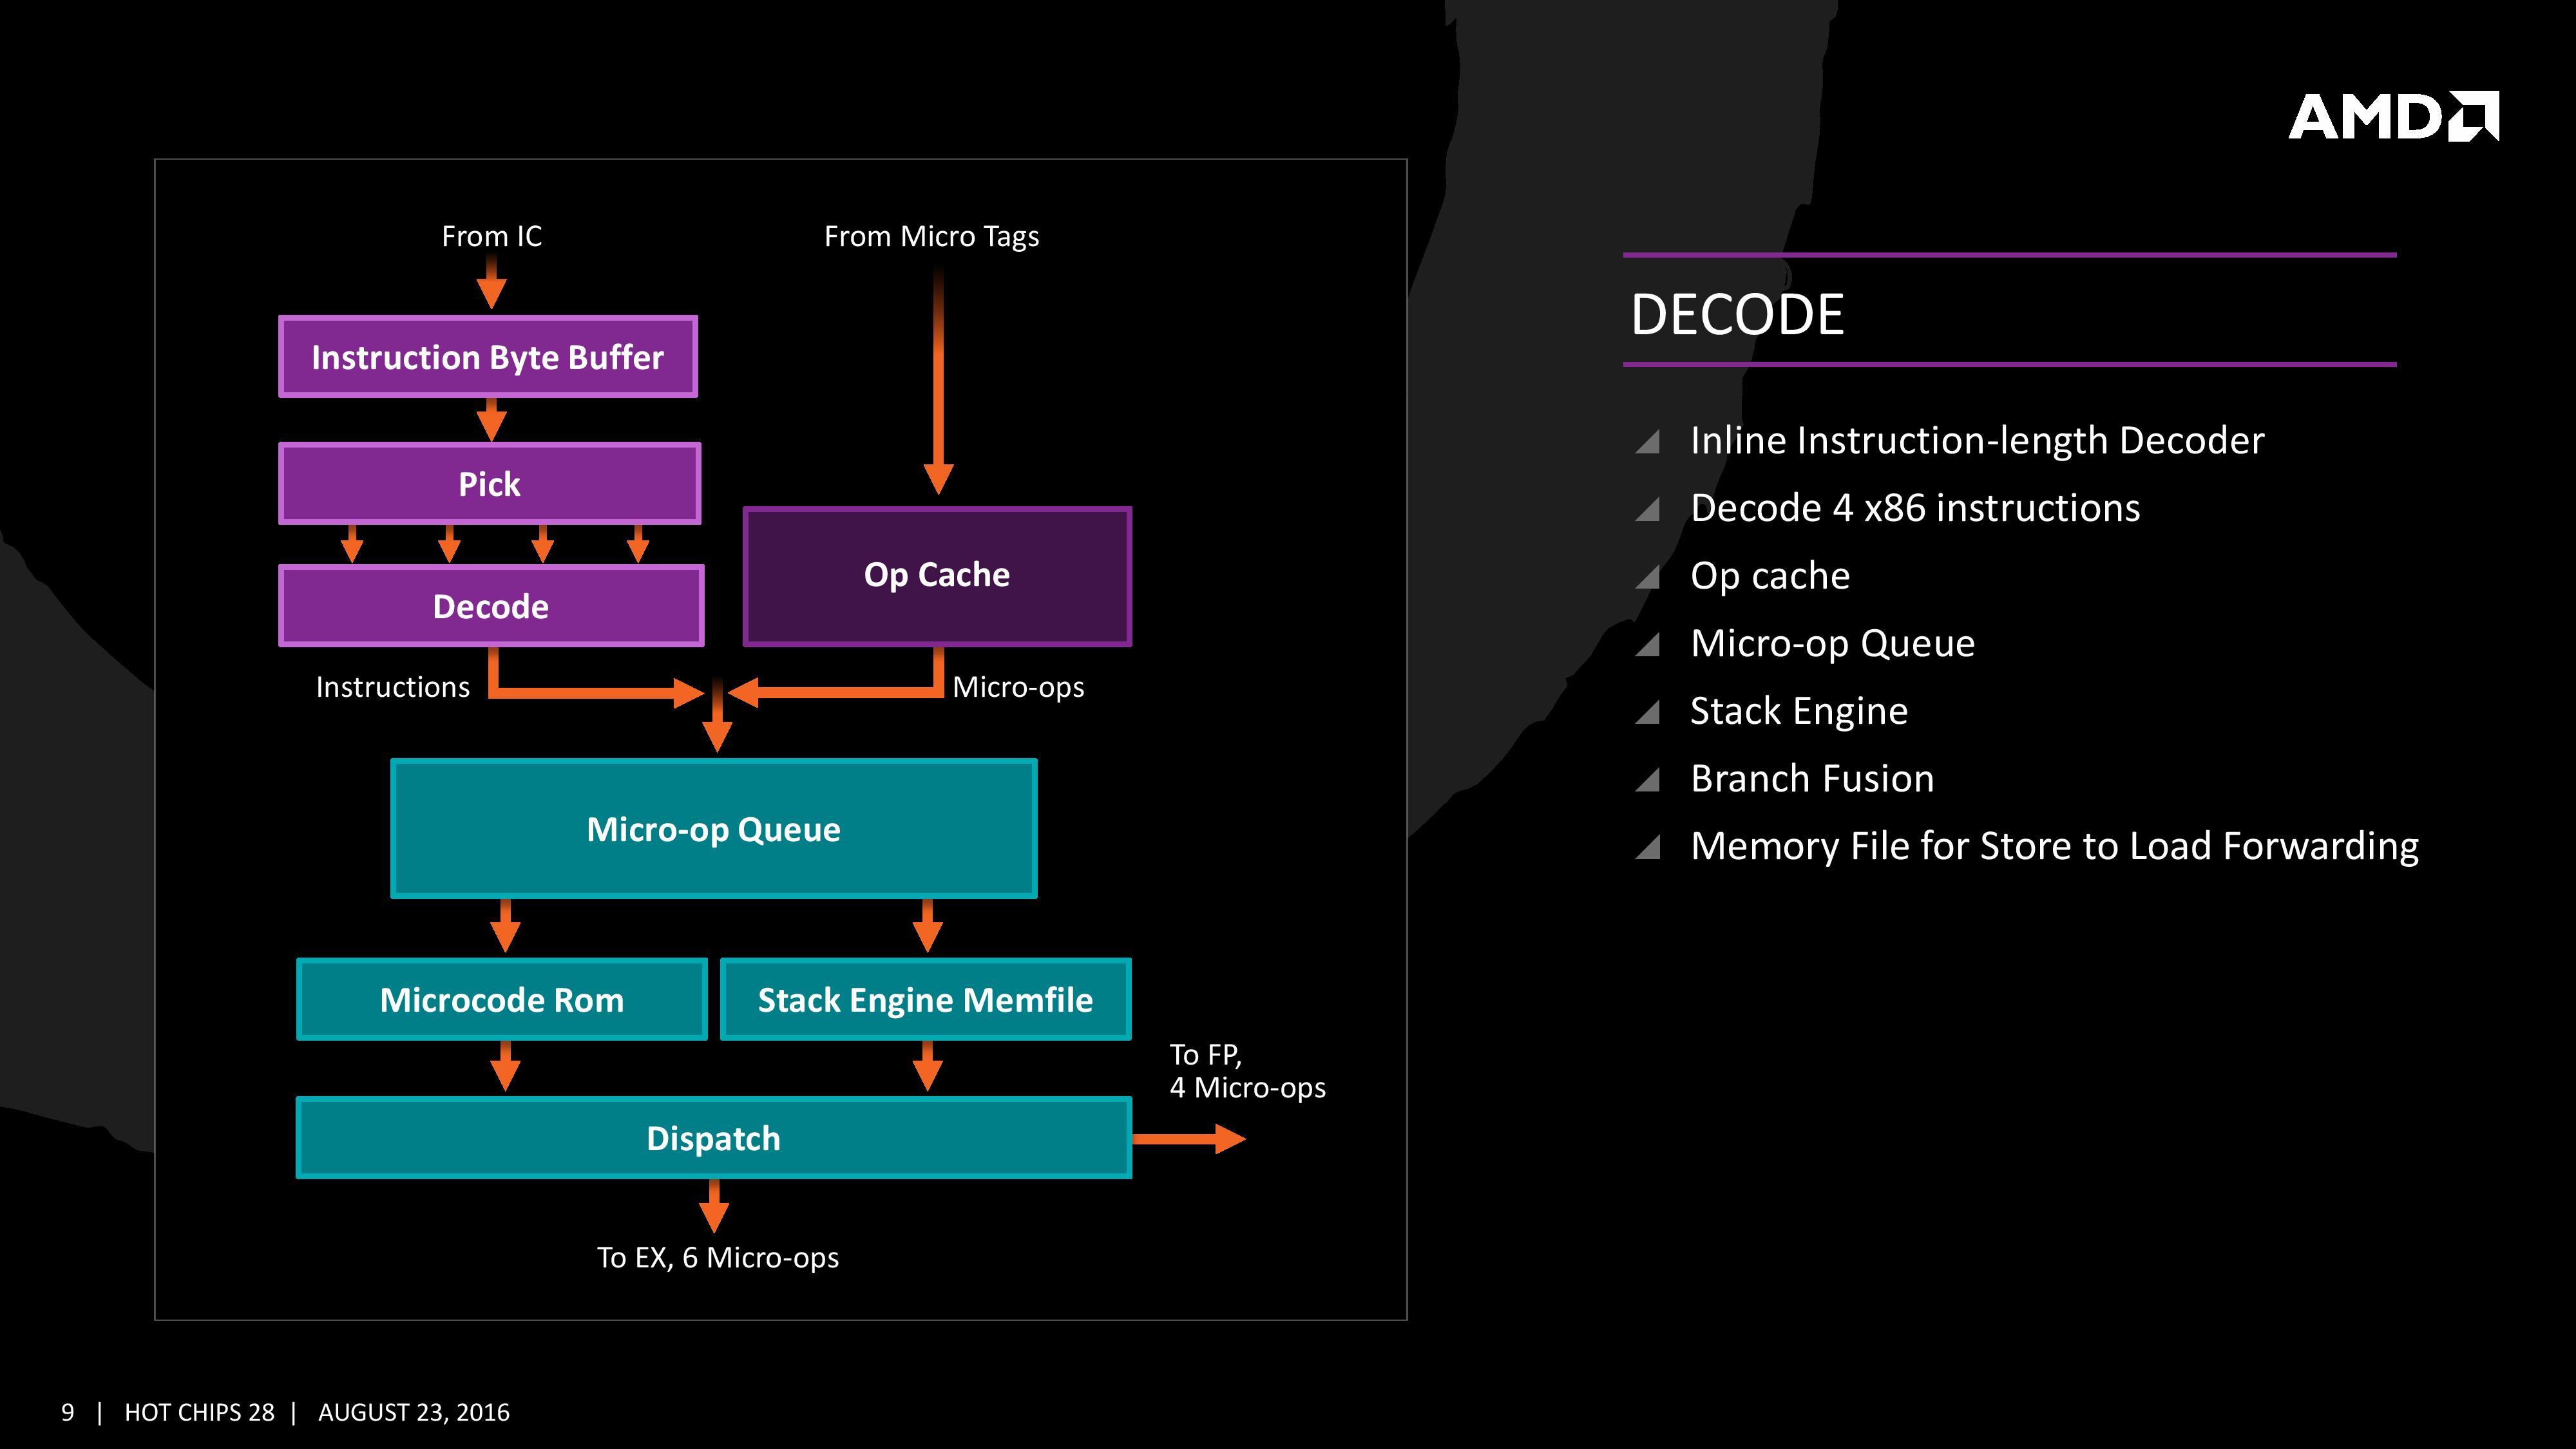
\includegraphics[width=115mm,scale=0.5]{amd-zen-decode.jpg}
\caption{CPU Complex, fonte: AMD}
\label{fig:AMD CORE}
\end{figure}

Na parte de decodificação, é interessante ressaltar a Stack Engine e o dispatch:
\begin{itemize}
	\item A Stack Engine aparece entre a queue e o dispatch(último bloco), permitindo uma geração de endereços de baixo-custo quando já é conhecido de ciclos anteriores. Isso permite que o sistema salve energia indo através da AGU e "percorrendo" as caches.
	\item O dispatch do ZEN pode aplicar seis instruções por clock, até um máximo de 6/ciclos para INT e 4/ciclos para FP.
\end{itemize}

\newpage

\section{General Information}

All full papers and posters (short papers) submitted to some SBC conference,
including any supporting documents, should be written in English or in
Portuguese. The format paper should be A4 with single column, 3.5 cm for upper
margin, 2.5 cm for bottom margin and 3.0 cm for lateral margins, without
headers or footers. The main font must be Times, 12 point nominal size, with 6
points of space before each paragraph. Page numbers must be suppressed.

Full papers must respect the page limits defined by the conference.
Conferences that publish just abstracts ask for \textbf{one}-page texts.

\newpage

\section{First Page} \label{sec:firstpage}

The first page must display the paper title, the name and address of the
authors, the abstract in English and ``resumo'' in Portuguese (``resumos'' are
required only for papers written in Portuguese). The title must be centered
over the whole page, in 16 point boldface font and with 12 points of space
before itself. Author names must be centered in 12 point font, bold, all of
them disposed in the same line, separated by commas and with 12 points of
space after the title. Addresses must be centered in 12 point font, also with
12 points of space after the authors' names. E-mail addresses should be
written using font Courier New, 10 point nominal size, with 6 points of space
before and 6 points of space after.

The abstract and ``resumo'' (if is the case) must be in 12 point Times font,
indented 0.8cm on both sides. The word \textbf{Abstract} and \textbf{Resumo},
should be written in boldface and must precede the text.

\newpage

\section{CD-ROMs and Printed Proceedings}

In some conferences, the papers are published on CD-ROM while only the
abstract is published in the printed Proceedings. In this case, authors are
invited to prepare two final versions of the paper. One, complete, to be
published on the CD and the other, containing only the first page, with
abstract and ``resumo'' (for papers in Portuguese).
\newpage
\section{Sections and Paragraphs}

Section titles must be in boldface, 13pt, flush left. There should be an extra
12 pt of space before each title. Section numbering is optional. The first
paragraph of each section should not be indented, while the first lines of
subsequent paragraphs should be indented by 1.27 cm.

\subsection{Subsections}

The subsection titles must be in boldface, 12pt, flush left.
\newpage
\section{Figures and Captions}\label{sec:figs}


Figure and table captions should be centered if less than one line
(Figure~\ref{fig:exampleFig1}), otherwise justified and indented by 0.8cm on
both margins, as shown in Figure~\ref{fig:exampleFig2}. The caption font must
be Helvetica, 10 point, boldface, with 6 points of space before and after each
caption.

\begin{figure}[H]
\centering
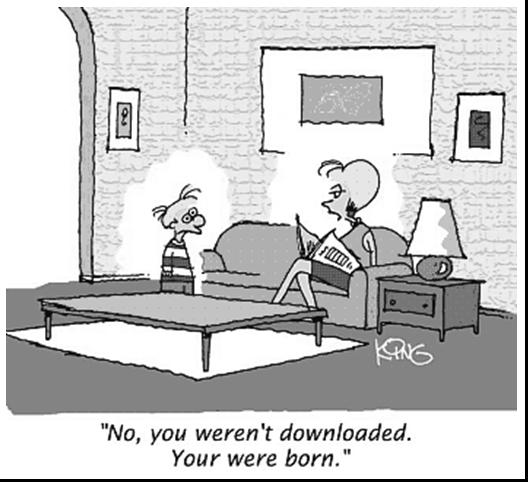
\includegraphics[width=.5\textwidth]{fig1.jpg}
\caption{A typical figure}
\label{fig:exampleFig1}
\end{figure}

\begin{figure}[H]
\centering
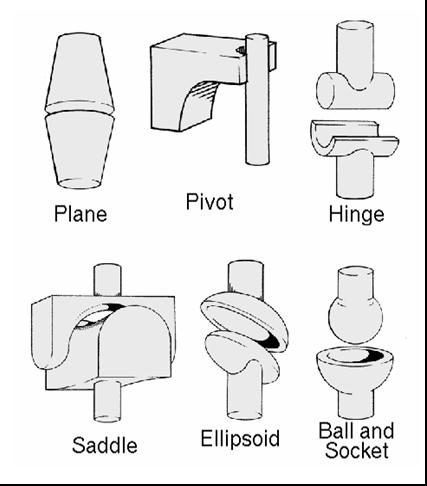
\includegraphics[width=.3\textwidth]{fig2.jpg}
\caption{This figure is an example of a figure caption taking more than one
  line and justified considering margins mentioned in Section~\ref{sec:figs}.}
\label{fig:exampleFig2}
\end{figure}

In tables, try to avoid the use of colored or shaded backgrounds, and avoid
thick, doubled, or unnecessary framing lines. When reporting empirical data,
do not use more decimal digits than warranted by their precision and
reproducibility. Table caption must be placed before the table (see Table 1)
and the font used must also be Helvetica, 10 point, boldface, with 6 points of
space before and after each caption.

\begin{table}[ht]
\centering
\caption{Variables to be considered on the evaluation of interaction
  techniques}
\label{tab:exTable1}
\smallskip
\begin{tabular}{|l|c|c|}
\hline
& Value 1 & Value 2\\[0.5ex]
\hline
&&\\[-2ex]
Case 1 & 1.0 $\pm$ 0.1 & 1.75$\times$10$^{-5}$ $\pm$ 5$\times$10$^{-7}$\\[0.5ex]
\hline
&&\\[-2ex]
Case 2 & 0.003(1) & 100.0\\[0.5ex]
\hline
\end{tabular}
\end{table}

\newpage

\section{Images}

All images and illustrations should be in black-and-white, or gray tones,
excepting for the papers that will be electronically available (on CD-ROMs,
internet, etc.). The image resolution on paper should be about 600 dpi for
black-and-white images, and 150-300 dpi for grayscale images.  Do not include
images with excessive resolution, as they may take hours to print, without any
visible difference in the result. 

\newpage

\section{References}

Bibliographic references must be unambiguous and uniform.  We recommend giving
the author names references in brackets, e.g. \cite{knuth:84},
\cite{boulic:91}, and \cite{smith:99}.

The references must be listed using 12 point font size, with 6 points of space
before each reference. The first line of each reference should not be
indented, while the subsequent should be indented by 0.5 cm.

\bibliographystyle{sbc}
\bibliography{sbc-template}

\end{document}
